% !TeX root = ../paper.tex
% !TeX encoding = UTF-8
% !TeX spellcheck = en_US

\section{Actor Memory Overhead Experiments}\label{sec:experiments}

  Our concept is based on the usage of hundreds of thousands of \glspl{dactor}, which all store only a small amount of data.
  This raises the question of how much memory overhead is introduced for storing data split across a multitude of actors.
  Therefore, we performed experiments comparing the memory usage of an exemplary actor database system with that of just loading the data into our data storage abstraction, called relations, or in a big string into memory.

\subsection{Experimental Setup}

  The exemplary actor database system used for testing consists of four different \gls{dactor} types, each containing different number of relations and data sizes.
  We used a script to generate four different datasets emulating the scaling of the system by increasing the number of \gls{dactor}-instances in the system and keeping the data size stored in one \gls{dactor} nearly constant.
  The script creates various primitive data types, such as \code{String}, \code{Double}, and \code{Int}, as well as complex data types, such as \code{ZonedDateTime}, and distributes the data across \glspl{dactor} and relations.
  The data distribution across the \gls{dactor} types is reported in \cref{tab:datasets:size_distribution} and the key figures of the datasets are reported in \cref{tab:datasets:keyfigures}.
  The data size stored in one \gls{dactor} and one relation is very small (in the kilobytes range), this will make the relative memory overhead more visible as we need thousands of \glspl{dactor} and relations to store our datasets in the heap.
  
  \begin{table}
    \centering
    \begin{subtable}[t]{0.445\textwidth}
      \centering
      \begin{tabular}{@{}crr@{}}
        \toprule
        \textbf{\Gls{dactor} type} & \textbf{Data size} & \textbf{\# Relations}\\
        \midrule
        $X_1$ &   7~KB & 2 \\ % Cart
        $X_2$ &  22~KB & 3 \\ % Customer
        $X_3$ & 171~KB & 2 \\ % StoreSection
        $X_4$ & 721~KB & 1 \\ % GroupManager
        \bottomrule
      \end{tabular}
      \subcaption{\Gls{dactor} types and their corresponding data sizes}
      \label{tab:datasets:size_distribution}
    \end{subtable}
    \begin{subtable}[t]{0.545\textwidth}
      \centering
      \begin{tabular}{@{}crrr@{}}
        \toprule
        \textbf{Dataset} & \textbf{Size on disk} & \textbf{\# \Glspl{dactor}} & \textbf{\# Relations}\\
        \midrule
        $D_1$ & 10~MB & 829 & 1~714 \\
        $D_2$ & 25~MB & 2~578 & 5~250 \\
        $D_3$ & 50~MB & 4~373 & 8~935 \\
        $D_4$ & 100~MB & 8~618 & 17~596 \\
        \bottomrule
      \end{tabular}
      \subcaption{Datasets sizes and key figures}
      \label{tab:datasets:keyfigures}
    \end{subtable}
    \caption{Datasets used for the memory overhead experiments}
    \label{tab:datasets}
  \end{table}

  For each dataset we performed three different tests:
  \begin{description}
    \item[\textit{Single string}] Convert all data into its \code{String} representation and load it as a single big \code{String} into memory.
      This test serves as baseline for the other ones.
    \item[\textit{Relations}] Load the data into their respective \code{Relation}s, preserving the type information and using the in-memory data storage objects from our framework.
    \item[\textit{Framework}] Use the full-fledged framework to load the data into memory.
      This approach stores the data distributed across \glspl{dactor} in \code{Relation} objects.
  \end{description}

  To obtain the used memory of the objects in our test approaches, we used VisualVM\footnote{\url{https://visualvm.github.io/}} to create heap dumps.
  After the data was completely loaded into memory, we triggered a garbage collection run and created a heap dump.
  VisualVM is able to compute the retained sizes of object hierarchies in those dumps.
  This allowed us to investigate the memory usage of selected objects and their members in detail.
  We report the results of those experiments in the next section and discuss them in \cref{sec:exp:discussion}.

\subsection{Results}

  \Cref{fig:exp:general} shows an overview about the measured heap size of the different tests over the four datasets.
  If the data is loaded into memory as a single big \code{String} object, it takes up around the same amount of heap as the dataset is big.
  Storing the data in \textit{Relations} introduces a overhead of about $150 \%$.
  % relations - string / string = ratio
  % 18162800 / 11315812 = 161%
  % 26453405 / 18637898 = 142%
  % 72695967 / 49246330 = 148%
  % 145392010 / 98492584 = 148%
  Even for the smallest dataset the data is split up across thousands of relations, which each use a two dimensional \code{Array} to store the individual values in a non-optimized way.
  In addition to that, relations also store metadata about the contained data, such as column names and data types.
  % show relations with more data stored than a couple kilobytes
  
  \begin{figure}
    \centering
    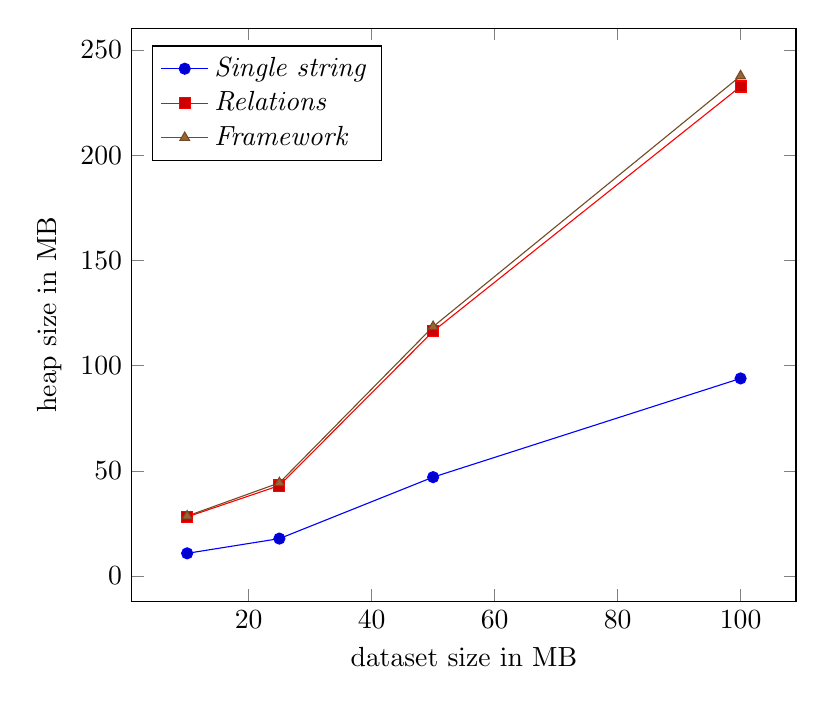
\begin{tikzpicture}
      \begin{axis}[
      scale only axis,
          xlabel=dataset size in MB,
          ylabel=heap size in MB,
          legend pos=north west,
          legend cell align={left},
      ]
        \addplot coordinates {
          (10,10.8) (25,17.8) (50,47.0) (100,93.9)
        };
        \addplot coordinates {
          (10,28.1) (25,43.0) (50,116.3) (100,232.6)
        };
        \addplot+[mark=triangle*] coordinates {
          (10,28.5) (25,44.3) (50,118.5) (100,237.6)
        };
        \legend{\textit{Single string}, \textit{Relations}, \textit{Framework}}
      \end{axis}
    \end{tikzpicture}
    \caption{Used heap size when loading the data into memory using the three different methods.}
    \label{fig:exp:general}
  \end{figure}

  As we can see in \cref{fig:exp:general}, using the full framework with \glspl{dactor} does not introduce much additional memory overhead.
  \Cref{tab:memory_overhead} compares the sizes of the \textit{Relations} and \textit{Framework} tests and lists the \gls{dactor} overhead for the datasets $D_1$ through $D_4$.
  The memory overhead per \gls{dactor} is computed with the following equation:
  \begin{equation}
    \text{Overhead / \gls{dactor}} = \frac{\text{Size \textit{Framework}} - \text{Size \textit{Relations}}}{\text{\# \glspl{dactor}}}
  \end{equation}
  In average, using a \gls{dactor} only needs an additional 533~B more.

  \begin{table}
    \centering
    \begin{tabular}{crrrr}
      \toprule
      \textbf{Dataset} & \textbf{\# \Glspl{dactor}} & \textbf{Size \textit{Relations}} & \textbf{Size \textit{Framework}} & \textbf{Overhead / \gls{dactor}}\\
      \midrule
      $D_1$ & 829 & 28~788~KB & 29~213~KB & 526~B \\
      $D_2$ & 2~578 & 44~034~KB & 45~392~KB & 539~B \\
      $D_3$ & 4~373 & 119~084~KB & 121~355~KB & 532~B \\
      $D_4$ & 8~618 & 238~169~KB & 242~728~KB & 534~B \\
      % Average overhead = 533B
      \bottomrule
    \end{tabular}
    \caption{Memory overhead of \glspl{dactor}}
    \label{tab:memory_overhead}
  \end{table}


\subsection{Discussion}\label{sec:exp:discussion}

  \Cref{tab:memory_overhead} clearly shows that using \glspl{dactor} only introduces a very small memory overhead.
  \Glspl{dactor} have a constant overhead of about 550~B per instance.
  Our experiments show a worst case scenario, where each \gls{dactor} only stores 230~KB on average.
  
  Lets assume, we have a 1~TB database and we chose to store 1~MB per \gls{dactor}.
  This requires the actor database to instantiate about one million \glspl{dactor}.
  Using the average overhead of 550~B per \gls{dactor}, this would yield a relative memory overhead of only $0.05~\%$.
  Doing the same thought experiment with storing 10~MB per \gls{dactor}, results in about 100~000 \glspl{dactor} and reduces the relative memory overhead to $0.005 \%$.

  During execution of the experiments, we noticed that the load times for the \textit{Framework} test were multiple times faster than the other testing scenarios.
  The data loading mechanism in the \textit{Framework} test is highly parallel, because each \gls{dactor} is responsible for loading its data.
  They are triggered by a initial message telling them, where to find the data.
